% !TEX program = xelatex
% Homework template

\documentclass[cn,12pt]{report}
% en is for English language
% cn is for Chinese language

%----- text fonts -----
%\usepackage[no-math]{fontspec}
%\usepackage{newtxtext}  % New TX font for text
%\setmainfont{TeX Gyre Termes}  % Times New Roman 的开源复刻版本
%\setsansfont{TeX Gyre Heros}   % Helvetica 的开源复刻版本
%\setmonofont{TeX Gyre Cursor}  % Courier New 的开源复刻版本
%\setmainfont{Times New Roman}
%\setsansfont{Arial}
%\setmonofont{Courier New}

%----- math font -----
%\usepackage{newtxmath}
%\usepackage{mathptmx}
%\usepackage{mathpazo}

%----- custom theorem -----
\newtheorem{innercustomgeneric}{\customgenericname}
\providecommand{\customgenericname}{}
\newcommand{\newcustomtheorem}[2]{%
  \newenvironment{#1}[1]
  {%
    \renewcommand\customgenericname{#2}%
    \renewcommand\theinnercustomgeneric{##1}%
    \innercustomgeneric
  }
  {\endinnercustomgeneric}
}

\newcustomtheorem{ntheorem}{定理}
\newcustomtheorem{nlemma}{引理}

%----- list style -----
\setlist{nolistsep}

% differential operator
\newcommand{\dif}{\mathop{}\!\mathrm{d}}

% new command
\newcommand{\CC}{\ensuremath{\mathbb{C}}}
\newcommand{\RR}{\ensuremath{\mathbb{R}}}
\newcommand{\A}{\mathcal{A}}
\newcommand{\bA}{\boldsymbol{A}}
\newcommand{\ii}{\mathrm{i}\,}
\newcommand{\dx}[1][x]{\mathop{}\!\mathrm{d}#1}
\newcommand{\abs}[1]{\lvert#1\rvert}
\newcommand{\norm}[1]{\left\lVert#1\right\rVert}
\newcommand{\red}[1]{\textcolor{red}{#1}}

%键入超链接
\usepackage{hyperref}
\hypersetup{hidelinks,
	colorlinks=true,
	allcolors=black,
	pdfstartview=Fit,
	breaklinks=true}

%----------------------------------------------------
%	HOMEWORK INFORMATION
%----------------------------------------------------

\header{\itshape 系统开发工具基础 -- 作业X  \quad 我是作业名字} % 页眉

\title{作业二 \quad Shell,Vim \& data cleaning} % 作业名字

\date{日期: \today} % 日期

\institute{中国海洋大学·信息科学与工程学部·计算机学院} % 学院或学校

\courseinfo{课程: 系统开发工具基础 } % 课程信息

\studentinfo{姓名: \textit{吴啸天} \quad 专业: \textit{计算机科学与技术} \quad 学号: 24020007137 \newline  \quad \href{https://github.com/Cheongfan/...}{Github: \quad https://github.com/Cheongfan/...}} % 学生信息

\begin{document}

\maketitle

%----------------------------------------------------
%	作业内容
%----------------------------------------------------

%\section*{作业题目}

%------------------------------%
\section{练习内容}
\subsection{内容简介}
  本次练习聚焦Shell命令行及脚本,Vim编辑器方法,以及一些数据整理方法,
  包括Shell 文件操作、函数编写与检索,Vim 基本编辑与配置,以及使用 cut、awk、sed 
  等工具进行数据提取、过滤、清洗与统计的内容,着重培养命令行工具的整合与实际数据处理能力。


\subsection{实例清单}
  1.【Shell】学习ls命令操作,按需输出目录列表。

  2.【Shell】编写marco 和 polo函数对工作目录进行两种方式的保存。

  3.【Shell】学习find命令查找所需文件名。

  4.【Shell】示例CSV文件的创建与验证。

  5.【Shell】按不同规则查询文件信息。

  6.【Shell】使用grep搜索特定内容,进行简单的搜索与过滤。

  7.【Shell】对文件进行复制与备份,并验证备份成功。

  8.【VIM】完成vimtutor下载安装。

  9.【VIM】下载 vimrc。

  10.【VIM】使用Vim创建.txt文件。

  11.【VIM】文件的搜索与替换 (单行)。
  
  12.【VIM】使用Vim进行全局搜索与替换。

  13.【Date\_leaning】使用cut命令提取特定列。

  14.【Date\_leaning】使用awk过滤特定行。

  15.【Date\_leaning】使用awk处理缺失值,将空年龄替换为0。

  16.【Date\_leaning】排序和去重操作。

  17.【Date\_leaning】使用awk进行高级格式化。

  18.【Date\_leaning】使用sed进行高级编辑,对标点符号进行操作,使用多个sed组合操作。

  19.【Date\_leaning】结合上文的计算、统计、查找命令,进行系统的数据分析。

  20.【Date\_leaning】创建和处理日志文件。
\section{解题感悟}
  在完成本次作业的过程中,我系统性地实践了 Shell 脚本编写、Vim 文本编辑及数据清洗等相关操作,进一步掌握了命令行环境下的高效工作流构建方法。通过编写 marco/polo 函数、使用 find/grep 进行文件查找与过滤、结合 awk/sed 完成结构化数据处理,我体会到命令行工具在自动化任务与数据处理方面的强大表达能力。尤其是在处理 CSV 文件和日志数据时,灵活组合文本处理命令能快速实现提取、过滤、转换与统计等功能,显著提升数据预处理的效率。

此外,Vim 的多种编辑模式与快捷键操作也让我意识到文本编辑器不仅限于输入,更是一个可高度定制的高效编程环境。经过本次练习,我对 Linux 环境下常用开发工具的使用有了更深刻的理解,也增强了解决实际工程中文件操作与数据清洗问题的信心。

\section{练习过程与成果}
  \begin{figure}[htbp]
    \centering
    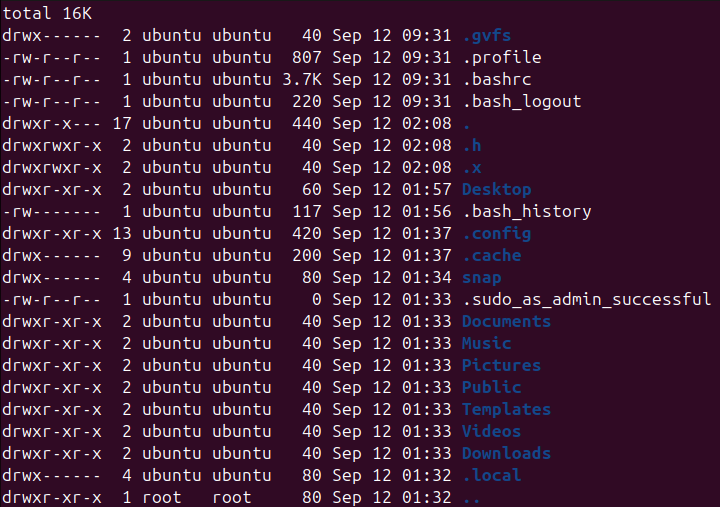
\includegraphics[width=1\textwidth]{image/1.png}
    \caption{实例1}
  \end{figure}

  \begin{figure}[htbp]
    \centering
    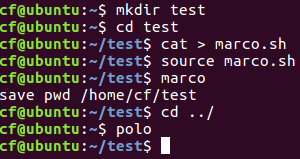
\includegraphics[width=1\textwidth]{image/2.png}
    \caption{实例2}
  \end{figure}

    \begin{figure}[htbp]
    \centering
    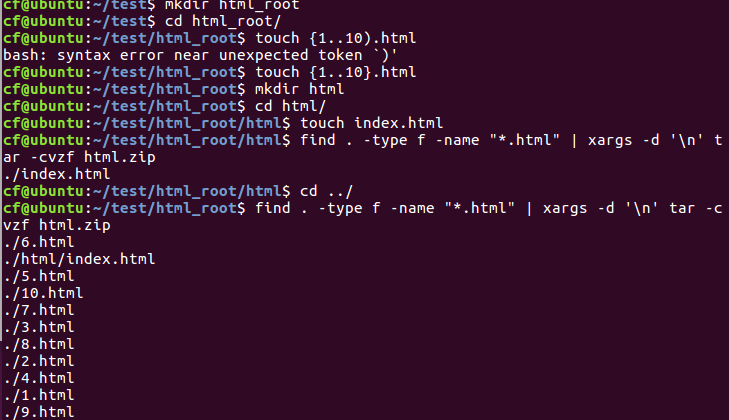
\includegraphics[width=1\textwidth]{image/3.png}
    \caption{实例3}
  \end{figure}

    \begin{figure}[htbp]
    \centering
    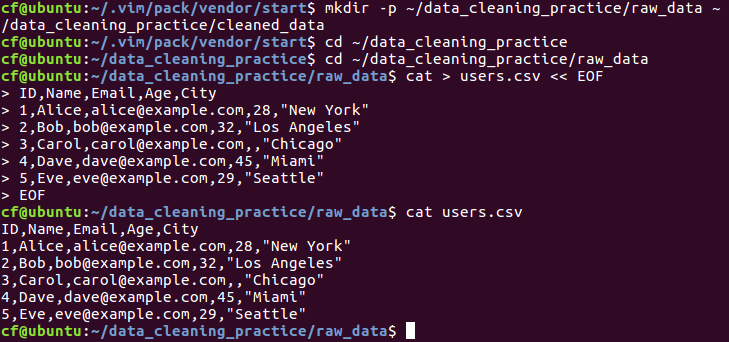
\includegraphics[width=1\textwidth]{image/4.png}
    \caption{实例4}
  \end{figure}

    \begin{figure}[htbp]
    \centering
    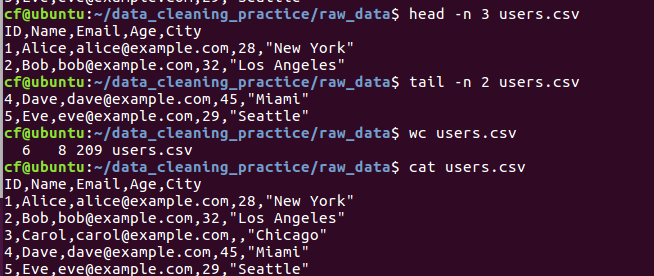
\includegraphics[width=1\textwidth]{image/5.png}
    \caption{实例5}
  \end{figure}

    \begin{figure}[htbp]
    \centering
    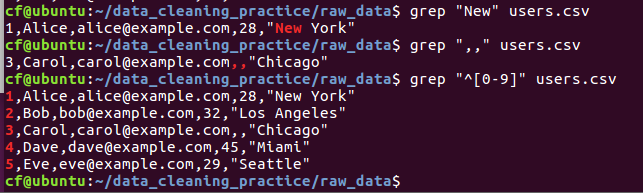
\includegraphics[width=1\textwidth]{image/6.png}
    \caption{实例6}
  \end{figure}

    \begin{figure}[htbp]
    \centering
    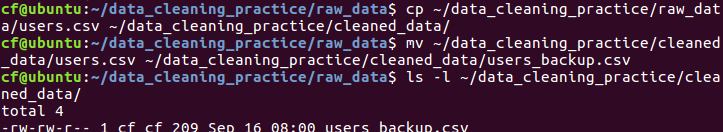
\includegraphics[width=1\textwidth]{image/7.png}
    \caption{实例7}
  \end{figure}

    \begin{figure}[htbp]
    \centering
    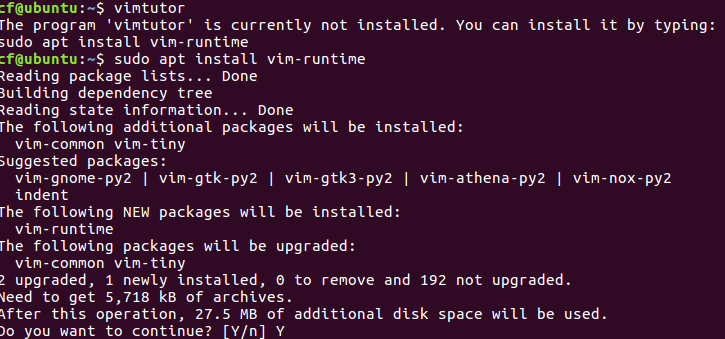
\includegraphics[width=1\textwidth]{image/8.png}
    \caption{实例8}
  \end{figure}

      \begin{figure}[htbp]
    \centering
    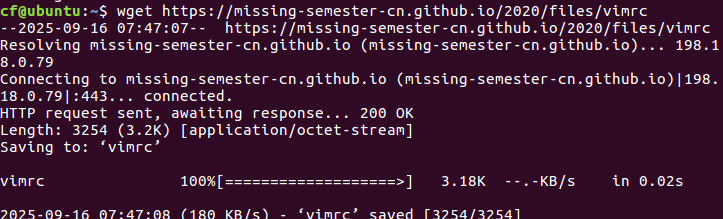
\includegraphics[width=1\textwidth]{image/9.png}
    \caption{实例9}
  \end{figure}

      \begin{figure}[htbp]
    \centering
    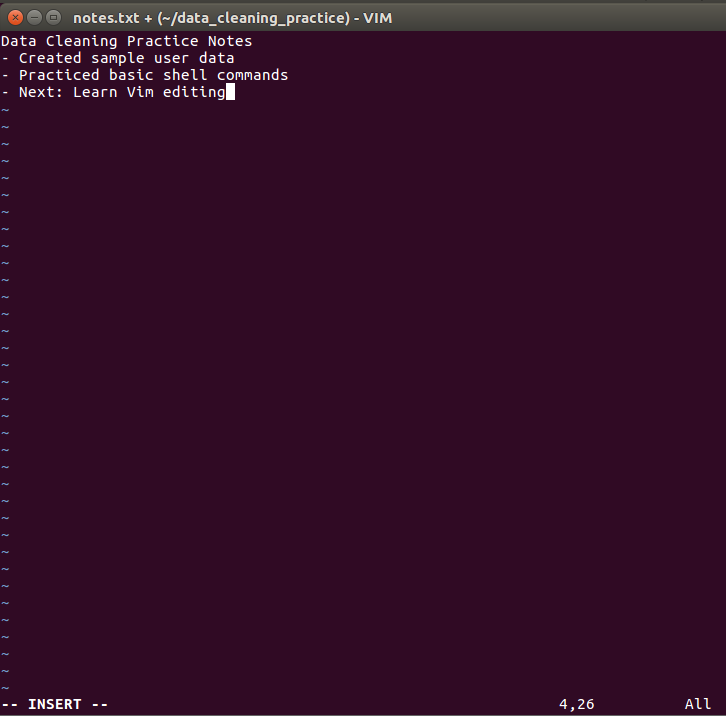
\includegraphics[width=1\textwidth]{image/10.png}
    \caption{实例10}
  \end{figure}

      \begin{figure}[htbp]
    \centering
    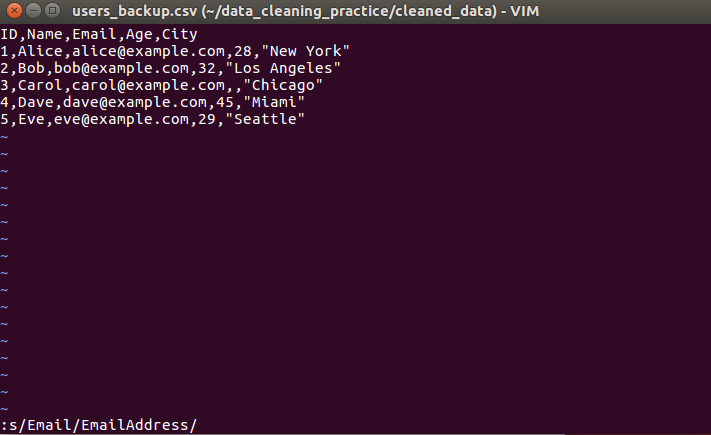
\includegraphics[width=1\textwidth]{image/11.png}
    \caption{实例11}
  \end{figure}

      \begin{figure}[htbp]
    \centering
    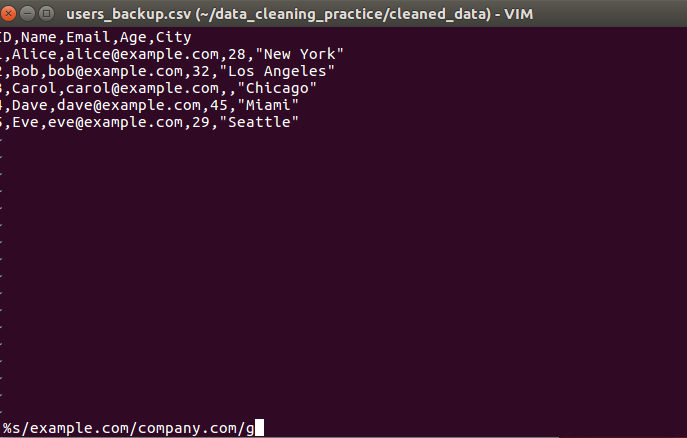
\includegraphics[width=1\textwidth]{image/12.png}
    \caption{实例12}
  \end{figure}

      \begin{figure}[htbp]
    \centering
    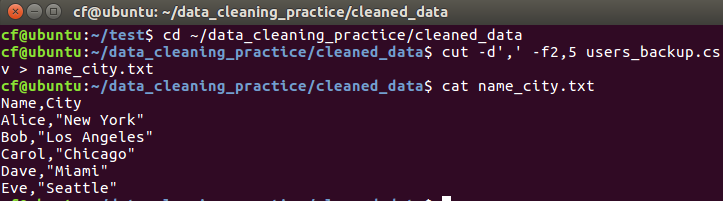
\includegraphics[width=1\textwidth]{image/13.png}
    \caption{实例13}
  \end{figure}

    \begin{figure}[htbp]
    \centering
    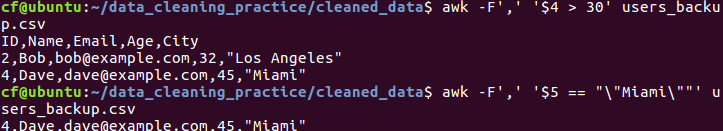
\includegraphics[width=1\textwidth]{image/14.png}
    \caption{实例14}
  \end{figure}

      \begin{figure}[htbp]
    \centering
    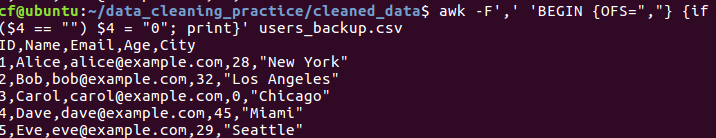
\includegraphics[width=1\textwidth]{image/15.png}
    \caption{实例15}
  \end{figure}

      \begin{figure}[htbp]
    \centering
    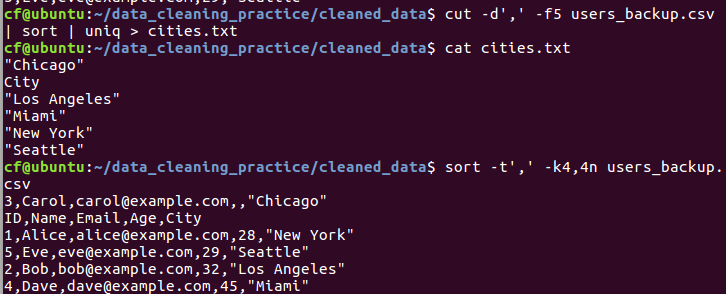
\includegraphics[width=1\textwidth]{image/16.png}
    \caption{实例16}
  \end{figure}

    \begin{figure}[htbp]
    \centering
    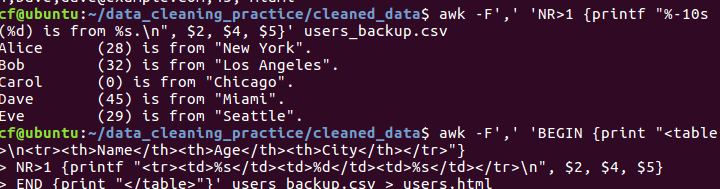
\includegraphics[width=1\textwidth]{image/17.png}
    \caption{实例17}
  \end{figure}

      \begin{figure}[htbp]
    \centering
    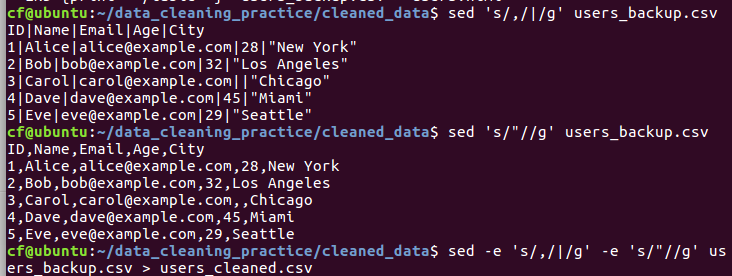
\includegraphics[width=1\textwidth]{image/18.png}
    \caption{实例18}
  \end{figure}

      \begin{figure}[htbp]
    \centering
    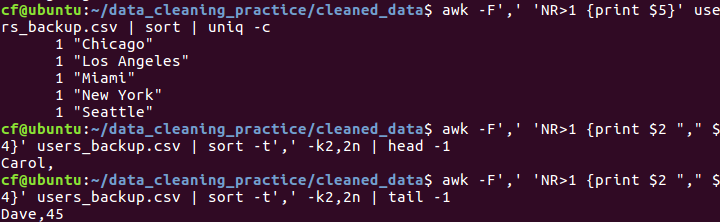
\includegraphics[width=1\textwidth]{image/19.png}
    \caption{实例19}
  \end{figure}

      \begin{figure}[htbp]
    \centering
    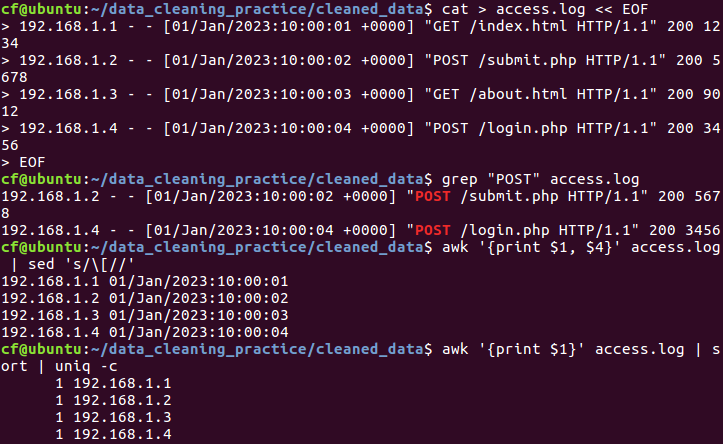
\includegraphics[width=1\textwidth]{image/20.png}
    \caption{实例20}
  \end{figure}

\newpage

\begin{thebibliography}{99}
\bibitem{这里是标签} https://blog.csdn.net/qq\_51247028/article/details/121180700
\bibitem{这里是标签} https://missing-semester-cn.github.io/missing-notes-and-solutions/2020/solutions/shell-tools-solution/
\bibitem{这里是标签} https://missing-semester-cn.github.io/missing-notes-and-solutions/2020/solutions/editors-solution/
\bibitem{这里是标签} https://missing-semester-cn.github.io/missing-notes-and-solutions/2020/solutions/shell-tools-solution/

\end{thebibliography}


\end{document}


